\documentclass[t,xcolor=pdftex,dvipsnames,table]{beamer}
\usepackage[]{graphicx}\usepackage[]{color}
%% maxwidth is the original width if it is less than linewidth
%% otherwise use linewidth (to make sure the graphics do not exceed the margin)
\makeatletter
\def\maxwidth{ %
  \ifdim\Gin@nat@width>\linewidth
    \linewidth
  \else
    \Gin@nat@width
  \fi
}
\makeatother

\definecolor{fgcolor}{rgb}{0.345, 0.345, 0.345}
\newcommand{\hlnum}[1]{\textcolor[rgb]{0.686,0.059,0.569}{#1}}%
\newcommand{\hlstr}[1]{\textcolor[rgb]{0.192,0.494,0.8}{#1}}%
\newcommand{\hlcom}[1]{\textcolor[rgb]{0.678,0.584,0.686}{\textit{#1}}}%
\newcommand{\hlopt}[1]{\textcolor[rgb]{0,0,0}{#1}}%
\newcommand{\hlstd}[1]{\textcolor[rgb]{0.345,0.345,0.345}{#1}}%
\newcommand{\hlkwa}[1]{\textcolor[rgb]{0.161,0.373,0.58}{\textbf{#1}}}%
\newcommand{\hlkwb}[1]{\textcolor[rgb]{0.69,0.353,0.396}{#1}}%
\newcommand{\hlkwc}[1]{\textcolor[rgb]{0.333,0.667,0.333}{#1}}%
\newcommand{\hlkwd}[1]{\textcolor[rgb]{0.737,0.353,0.396}{\textbf{#1}}}%
\let\hlipl\hlkwb

\usepackage{framed}
\makeatletter
\newenvironment{kframe}{%
 \def\at@end@of@kframe{}%
 \ifinner\ifhmode%
  \def\at@end@of@kframe{\end{minipage}}%
  \begin{minipage}{\columnwidth}%
 \fi\fi%
 \def\FrameCommand##1{\hskip\@totalleftmargin \hskip-\fboxsep
 \colorbox{shadecolor}{##1}\hskip-\fboxsep
     % There is no \\@totalrightmargin, so:
     \hskip-\linewidth \hskip-\@totalleftmargin \hskip\columnwidth}%
 \MakeFramed {\advance\hsize-\width
   \@totalleftmargin\z@ \linewidth\hsize
   \@setminipage}}%
 {\par\unskip\endMakeFramed%
 \at@end@of@kframe}
\makeatother

\definecolor{shadecolor}{rgb}{.97, .97, .97}
\definecolor{messagecolor}{rgb}{0, 0, 0}
\definecolor{warningcolor}{rgb}{1, 0, 1}
\definecolor{errorcolor}{rgb}{1, 0, 0}
\newenvironment{knitrout}{}{} % an empty environment to be redefined in TeX

\usepackage{alltt}
\newcommand{\SweaveOpts}[1]{}  % do not interfere with LaTeX
\newcommand{\SweaveInput}[1]{} % because they are not real TeX commands
\newcommand{\Sexpr}[1]{}       % will only be parsed by R


%\documentclass[handout,t,xcolor=pdftex,dvipsnames,table]{beamer}  % For handout
\mode<presentation>{
\useoutertheme[subsection=false]{miniframes}
%\beamertemplatenavigationsymbolsempty
\usecolortheme{custom}
\usefonttheme[onlymath]{serif}
\setbeamercovered{invisible}
%\setbeamertemplate{navigation symbols}{}
%\setbeamertemplate{mini frames}{}  % Old one
% Comment out this line to give the header
% \setbeamertemplate{headline}[default]
\setbeamertemplate{caption}[numbered]
%\setbeamertemplate{itemize items}[circle] 
\setbeamertemplate{frametitle continuation}{\frametitle{\color{white}Title}}  % So no tile on subsequent frames, from [allowframebreaks]

%%% CUSTOMISING NAVIATION %%%%
%This customises the navigation to be thin width and just have section headings (not subsections). 
\setbeamertemplate{headline}{%
\leavevmode%
  \hbox{%
    \begin{beamercolorbox}[wd=\paperwidth,ht=2.5ex,dp=1.125ex]{palette tertiary}%   % Tertiary colour is blue
    \insertsectionnavigationhorizontal{\paperwidth}{}{\hskip0pt plus1filll}
    \end{beamercolorbox}%
}}}

\RequirePackage{marvosym}

%%% INCLUDING SOLUTIONS %%%%
%% You can incorporate both questions and solutions in the 
%% same document.  Solutions can be included between the 
%% commands \begin{soln} and \end{soln}
%% To generate a pdf with only the questions uncomment:
%\excludecomment{soln}
\usepackage{comment}
\specialcomment{soln}{\begingroup \vspace{1mm} \sl}{ \leavevmode \endgroup}

%%%% DETAILS FOR PART 1 TITLE PAGE (OLD) %%%%
%\title{\large Part2 - Probability \& Distribution Theory} 
%\subtitle{} 
%\author{\copyright Dr Di Warren 2016} 
%\date{MATH1005 - Statistics}
% \colorlet{Faculty}{Arts}
%\colorlet{Faculty}{MasterBrandRed} % This is only needed if the notes are used for different faculties.
%\colorlet{FacultyText}{White}
% Defines the color of the text used on the title page and ``blocks''
% White for Business; TitlePageBlack for Arts, Pharmacy and Science
%\definecolor{CoolBlack}{rgb}{0.0, 0.18, 0.39}

%%%% DETAILS FOR FULL COURSE TITLE PAGE %%%%
\title{\Huge STATISTICS} 
\subtitle{} 
\author{\copyright University of Sydney 2017 (Di Warren)} 
\date{MATH1005}
% \colorlet{Faculty}{Arts}
\colorlet{Faculty}{MasterBrandRed} % This is only needed if the notes are used for different faculties.
\colorlet{FacultyText}{White}
% Defines the color of the text used on the title page and ``blocks''
% White for Business; TitlePageBlack for Arts, Pharmacy and Science
\definecolor{CoolBlack}{rgb}{0.0, 0.18, 0.39}

%%%% PACKAGES %%%%
\usepackage{multirow}
\usepackage{fancybox}
\usepackage[english]{babel}
\usepackage[utf8]{inputenc}
\usepackage{bm}
\usepackage{array}
\usepackage{booktabs}
\usepackage{tikz}
\usetikzlibrary{matrix,arrows,decorations.pathmorphing}
\usepackage{verbatim}
\usepackage{pgf,pgfsys,pgffor}
\usepackage{pgfplots}
\pgfplotsset{compat=1.3} %Recommended as of Pgfplots 1.3 - necessary?
\usetikzlibrary{decorations.pathreplacing,calc}
\usetikzlibrary{shapes, backgrounds}   % For Venn diagrams
\def \setA{ (0,0) circle (1cm) }
\def \setB{ (1.5,0) circle (1cm) }
\def \setC{ (0.6,1.5) circle (1cm) }
\def \setO{ (-2, -1.5) rectangle (3.5, 2.75) }
\tikzstyle{every picture}+=[remember picture]
\tikzstyle{na} = [baseline=-.5ex]
\usepackage{listings}  %Added by Di for adding R code

%\AtBeginSection[]
%{
%   \begin{frame}
 %      \frametitle{Outline}
 %      \tableofcontents[currentsection]
%   \end{frame}
%}  %This seems overkill for weekly lecture slides.

%\AtBeginSection[]
%{
%  \begin{frame}
% \frametitle{Contents}
%  \tiny{\tableofcontents[currentsection]}
%  \end{frame}
%}
%\useoutertheme{infolines} % Just lists current section in navigation at top, nice but limiting?

%%%% TITLE PAGE AND CONTENTS AT BEGINNING OF EACH TOPIC %%%%

\RequirePackage{ifthen} % package required
\newboolean{sectiontoc}
\setboolean{sectiontoc}{true} %default to true

\AtBeginSection[]
{
\begin{frame}[plain]
\vspace{60pt}
\begin{center}
\Huge{{\textcolor{MasterBrandBlue} \insertsection}}
\end{center}
\begin{tikzpicture}[scale=0.54]
%\hspace{-12pt}
%% Big Rectangle
\fill[MasterBrandRed] (0,14) -- (20,14) -- (20,15) -- (0,15);

%\draw (1,14.5) node [anchor = west] {\textcolor{MasterBrandBlue}{\Huge{\insertsection}}}; Overlays box with title, but long titles drop off the page
\end{tikzpicture} 
\end{frame}

%%%%%WORKING VERSION OF TOC%%%%%
%\begin{frame}
%   \frametitle{Outline}
%  \tableofcontents[currentsection, sectionstyle=show/hide, subsectionstyle=show/show/hide]
%  \end{frame}
%}

%%%%%2 VERSIONS - WITH AND WITHOUT TOC%%%%%
  \ifthenelse{\boolean{sectiontoc}}{
    \begin{frame}
  \frametitle{Outline}
  \tableofcontents[currentsection, sectionstyle=show/hide, subsectionstyle=show/show/hide]
 \end{frame}
  }
}
%%%%%This doesnt seem to work?%%%%
\newcommand{\toclesssection}[1]{
  \setboolean{sectiontoc}{false}
  %\section{#1}
  \setboolean{sectiontoc}{true}
}


% PDF settings
%\hypersetup{%
%  pdftitle={\inserttitle \insertsubtitle},%
%  pdfauthor={Di Warren},%
%	pdfsubject={},%
%	pdfkeywords={}%   
%	 }

%%%%  HELPFUL MACROS %%%%
\newcommand{\ud}{\mathrm{d}}
\newcommand{\var}{\mathrm{var}}
\newcommand{\ep}{\varepsilon}
\newcommand{\cov}{\mathrm{cov}}
\newcommand{\tr}{\mathrm{tr}}
\newcommand{\MSE}{\mathrm{MSE}}
\newcommand{\rank}{\mathrm{rank}}
\newcommand{\Bias}{\mathrm{Bias}}
\newcommand{\dei}{\partial}
\newcommand{\E}{\mathbb{E}}
\newcommand{\N}{\mathcal{N}}
\newcommand{\bbR}{\mathbb{R}}
\newcommand{\V}{\mathbb{V}}
\newcommand{\betahat}{\hat{\beta}}
\newcommand{\CLRM}{$\mathbf{y} = X\bm{\beta} + \bm{\ep}$}

%%%% LOGO FOR SLIDES %%%%
\logo{\vspace{79mm}
\includegraphics[height=0.9cm]{../images/sydney.pdf}}

%%%% ADD PAGE NUMBER %%%%
\setbeamertemplate{sidebar right}{}
\setbeamertemplate{footline}{%
\hfill\usebeamertemplate***{navigation symbols}
\hspace{1cm}\insertframenumber{}/\inserttotalframenumber}

%%%% BEGIN CONTENT %%%


\begin{document}



%%% TOPIC3 %%%%
\section[3]{Topic3: Bivariate Data}

\subsection[]{Example: Male Olympic 100m sprints}
\begin{frame}[fragile]{Example: Male Olympic 100m sprints}

The Male 100 metres sprint race in the Olympics is one of the most prestigious events in Athletics. The reigning champion is often named `the fastest man in the world', currently the Jamaican Usain Bolt. 

\vspace{.5cm}
{\bf Are the times getting faster in each Olympics? What would you predict the time for the next Olympics?}

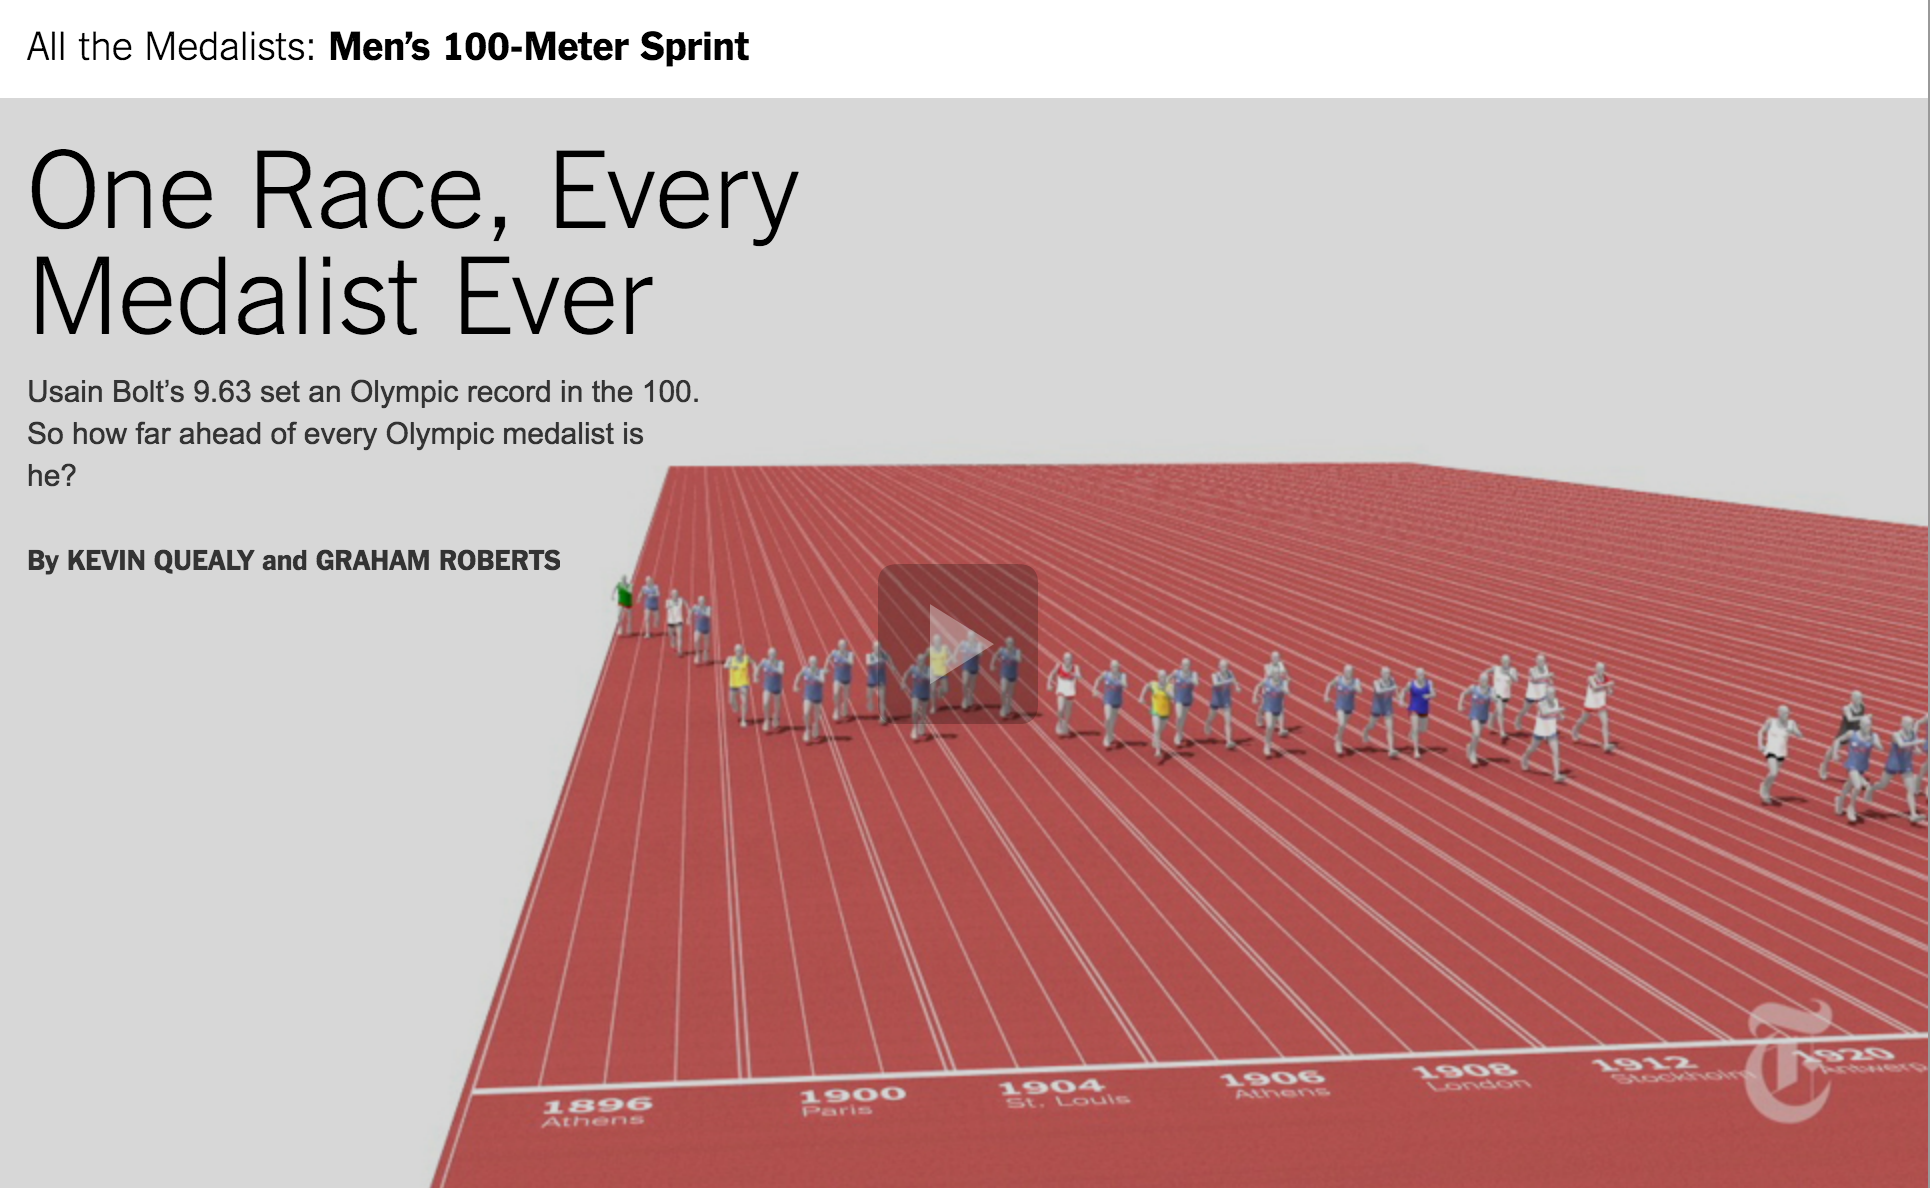
\includegraphics[height=3cm]{../images/Olympics100m.jpg}
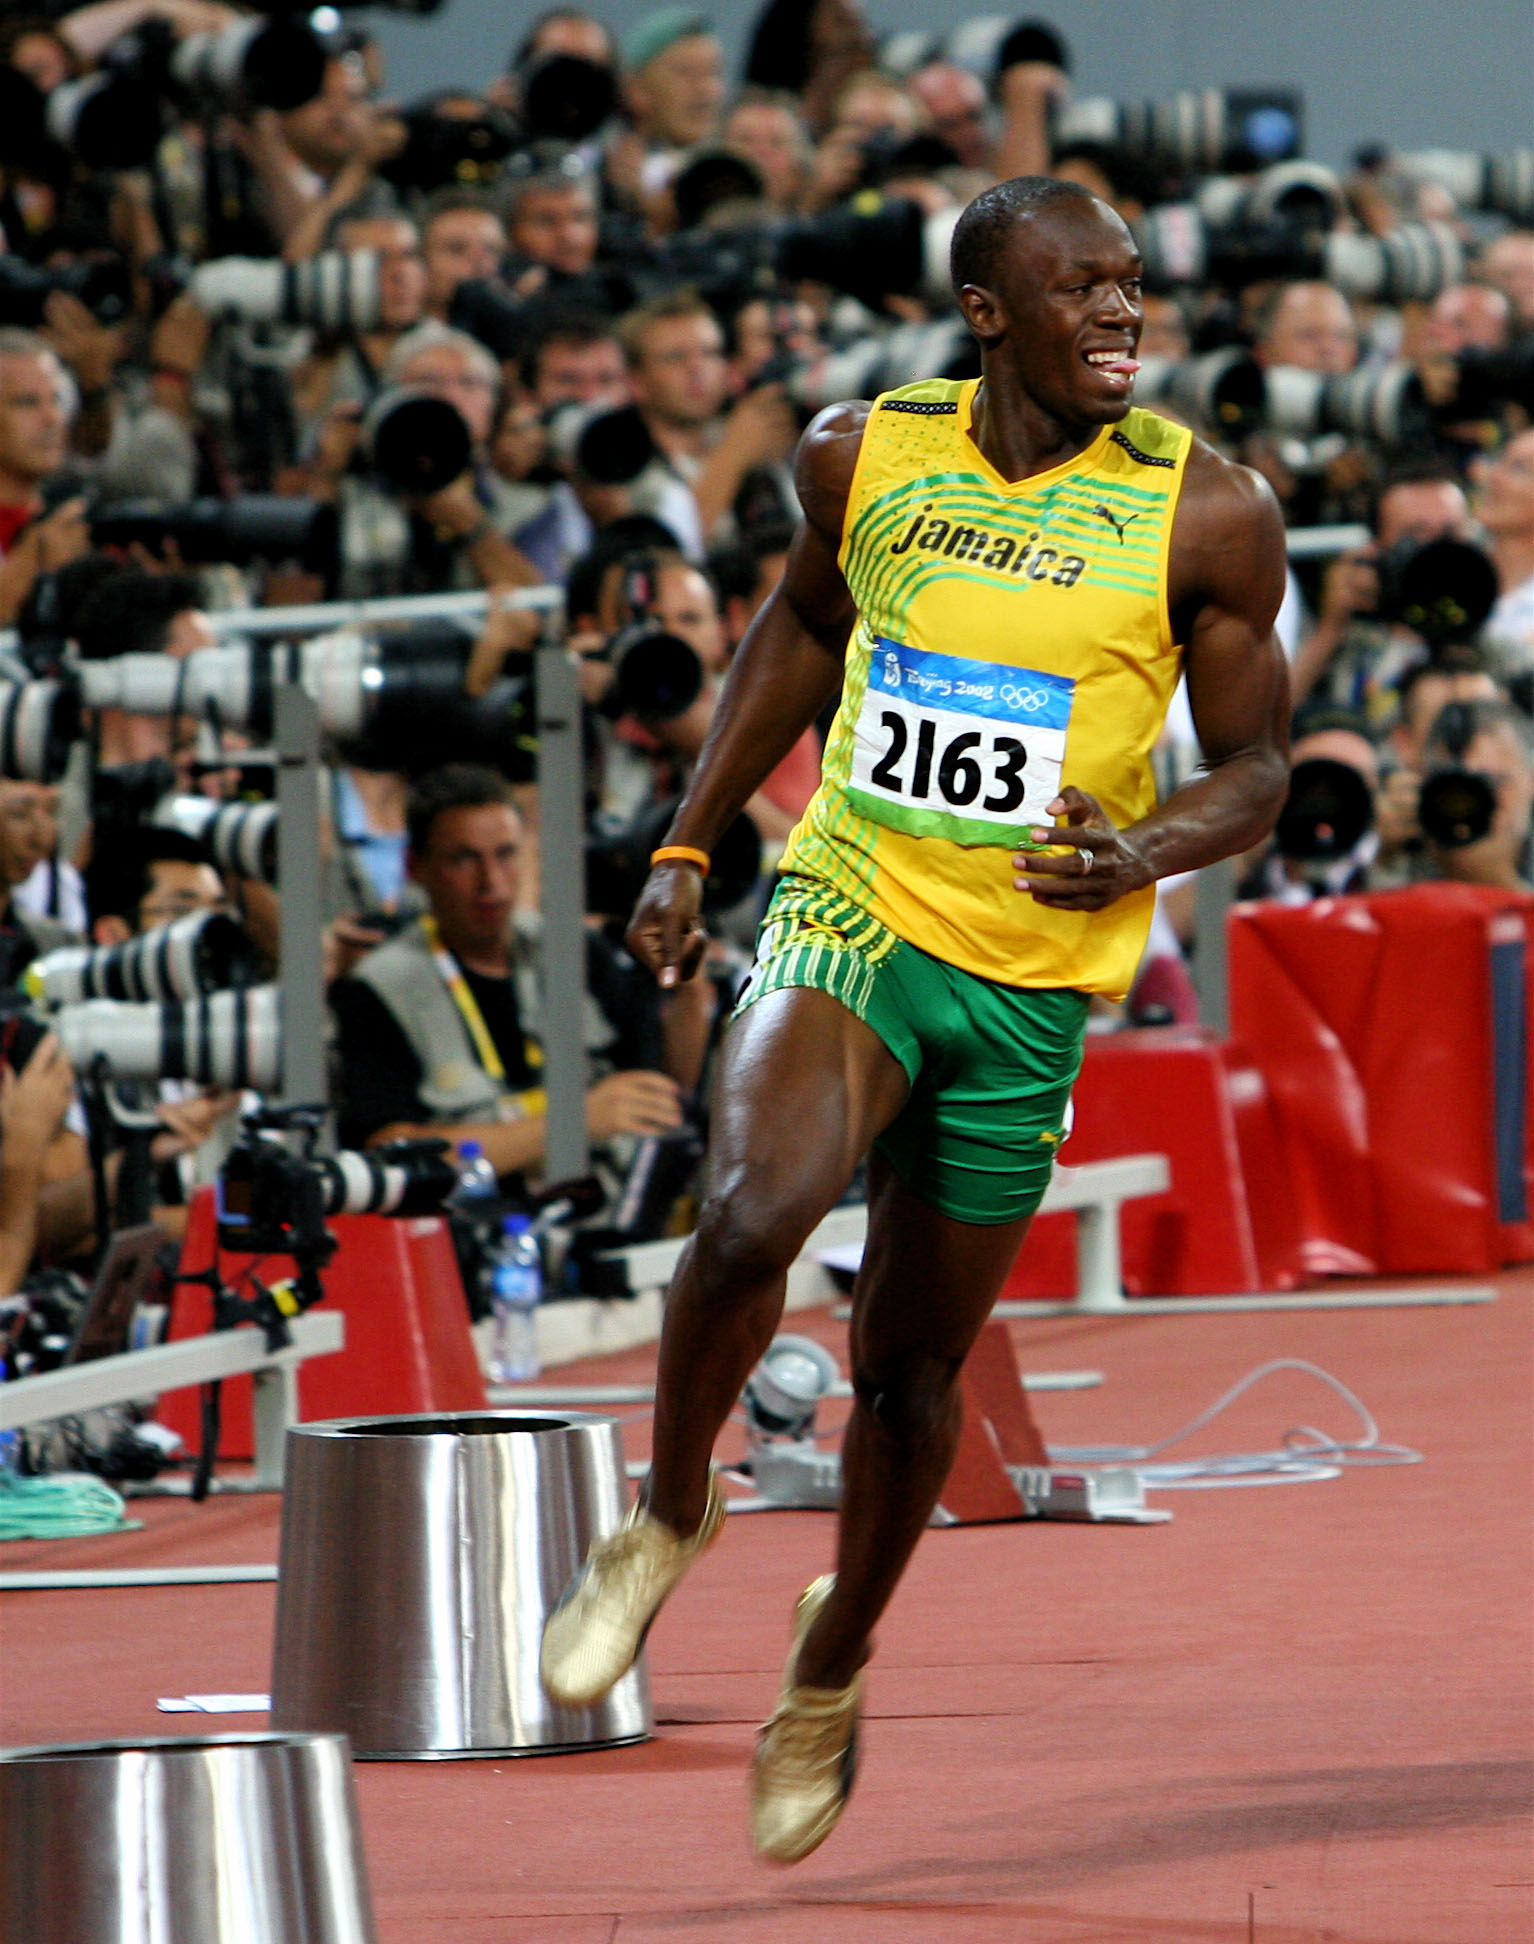
\includegraphics[height=5cm]{../images/UsainBolt.jpg}

\href{http://www.nytimes.com/interactive/2012/08/05/sports/olympics/the-100-meter-dash-one-race-every-medalist-ever.html}{\beamergotobutton{Olympics100mData}}
\end{frame}

\subsection[]{Bivariate Data}
\begin{frame}[fragile]{Bivariate Data}
In most contexts we collect many pieces of information for each ‘individual’ in the data set and look at the relationships between the variables (eg age, height, weight and income for USyd students).  This is called multivariate data.

\begin{itemize}
\item
We just consider bivariate data, of the form: $\{ (x_i,y_i) \}$ for  $i=1,2, \ldots, n$.

\item
$X$ is called the independent variable (or explanatory variable, predictor or regressor) and $Y$ is called the dependent variable (or response variable). These are determined by the context of the data.
\end{itemize}
\end{frame}

\subsection[]{Fitting a Least Squares Regression Model}
\begin{frame}[fragile]{Fitting a Model}
We are interested in fitting a model $Y = f(X) + error$, where the error is independent of the function $f(X)$ and follows a Normal curve (See Topic 6).

\begin{itemize}
\item
Examples include
$Y = \alpha + (X+\beta)^2 + \gamma + error$ (quadratic) or $Y=\alpha e^{\beta X}$ (exponential) or $Y=\alpha X^{\beta}$ (allometric).

\item
We will just consider the linear model: $Y = \alpha + \beta X + error$. 

\item
We use the sample values $\{ (x,y) \}$ to find an estimate of the model:
$y = a + b x + residual$.

\item
Note that both the exponential and allometric models can be expressed as a linear model by taking logs of each side.
\end{itemize}
\end{frame}



\begin{frame}[fragile]{Fitting a Linear Regression (LSL)}
Consider the following 5 steps:  
\begin{enumerate}

\item 
Construct a Scatterplot: $y$ vs $x$.

\item
If the plot looks linear, fit the Least Square’s (Regression) Line (LSL): $\hat{y} = a + b x$. 

\item
Construct a residual plot: $res= y-\hat{y} = y-(a+bx)$ vs $x$

\item
If the residual plot looks random, calculate the coefficient of determination ($r^2$) and correlation coefficient ($r$).

\item
Work out predictions for $y$, by finding $\hat{y}$ for a certain given $x$.
\end{enumerate}
\end{frame}


\subsection[]{Step1: Construct a Scatter plot}
\begin{frame}[fragile]{Step1: Construct a Scatter plot}
The 1st step is to construct a scatterplot of $Y$ vs $X$. This is a graphical summary of the bivariate data.

\vspace{.5cm}
This is 1st diagnostic: does the plot suggest a linear relationship between $Y$ and $X$, or not?
\end{frame}

\begin{frame}[fragile]{}
\begin{knitrout}
\definecolor{shadecolor}{rgb}{0.969, 0.969, 0.969}\color{fgcolor}\begin{kframe}
\begin{alltt}
\hlcom{## olympics <- read.csv("Olympics100m.csv",header=T)}
\hlstd{year}\hlkwb{=}\hlkwd{c}\hlstd{(olympics}\hlopt{$}\hlstd{Year)}
\hlstd{time}\hlkwb{=}\hlkwd{c}\hlstd{(olympics}\hlopt{$}\hlstd{Time)}
\hlkwd{plot}\hlstd{(year,time,} \hlkwc{xlab}\hlstd{=}\hlstr{"year"}\hlstd{,} \hlkwc{ylab}\hlstd{=}\hlstr{"time"}\hlstd{,}
     \hlkwc{main}\hlstd{=}\hlstr{"Olympics 100m 1968-2012"}\hlstd{)}
\end{alltt}
\end{kframe}
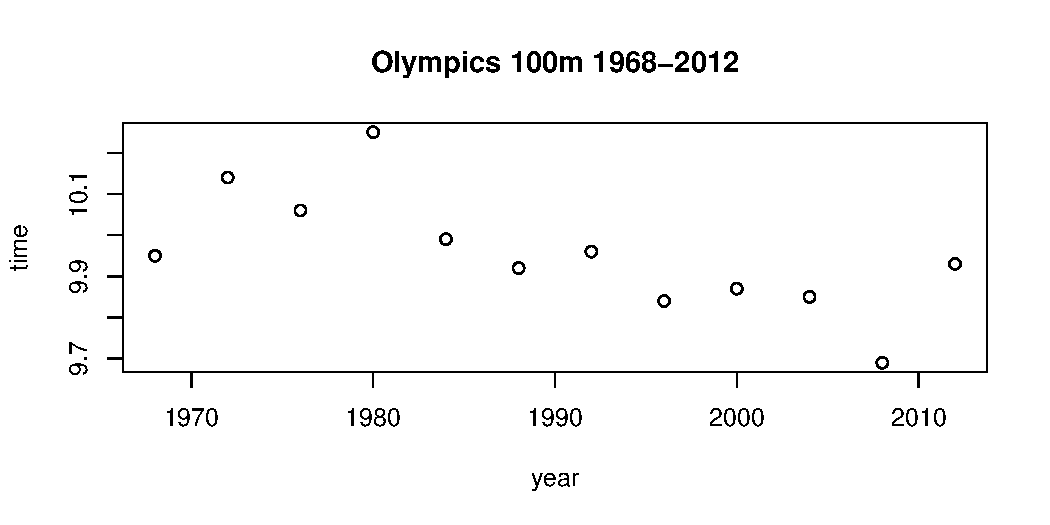
\includegraphics[width=\maxwidth]{figure/unnamed-chunk-2-1} 

\end{knitrout}
\end{frame}


\subsection[]{Step2: Fit the Least Square’s Line (LSL)}
\begin{frame}[fragile]{Step2: Fit the Least Square’s Line (LSL)}
If the scatter plot looks linear, then we fit the Least Square’s Regression Line (LSL).

\begin{itemize}
\item By `eye’, there are many possible lines, which could be drawn on the scatter plot – but which one is optimal?

\begin{knitrout}
\definecolor{shadecolor}{rgb}{0.969, 0.969, 0.969}\color{fgcolor}
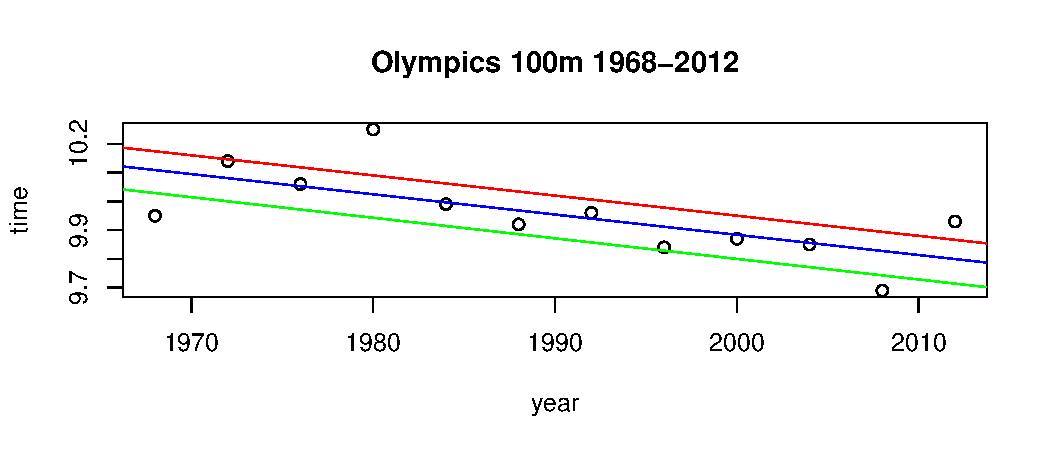
\includegraphics[width=\maxwidth]{figure/unnamed-chunk-3-1} 

\end{knitrout}
\end{itemize}
\end{frame}


\begin{frame}[fragile]{}
\begin{itemize}

\item 
For each candidate line $f(x)= a+bx$ for all $a$ and $b$, we focus on the resultant set of residuals: $res = e(a,b) = y-(a+bx)$. 

\vspace{.5cm}
This is the gaps between the line and the actual points.
For example, in the plot below the green residual is -0.1581 and the purple residual is 0.22603.
\end{itemize}

\begin{knitrout}
\definecolor{shadecolor}{rgb}{0.969, 0.969, 0.969}\color{fgcolor}
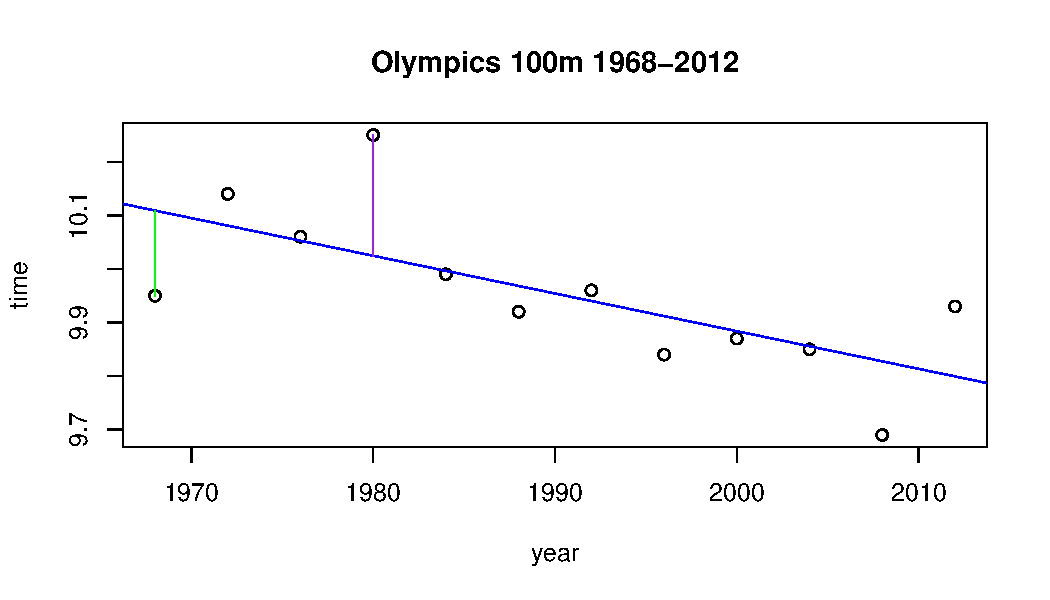
\includegraphics[width=\maxwidth]{figure/unnamed-chunk-4-1} 

\end{knitrout}
\end{frame}

\begin{frame}[fragile]{}

\begin{itemize}
\item   
We consider the `best’ line, to have the smallest residuals, determined by their sum of squared residuals 
\[ S(a,b)= \sum_{i=1}^{n} e(a,b)^2 = \sum_{i=1}^{n} (y - (a+bx))^2 \]

\item   
We minimise $S(a,b)$  by solving  $\frac{ \partial}{\partial a} = 0$ and 
$\frac{ \partial}{\partial b} = 0$. This gives 
 \[ \sum_{i=1}^{n} y_{i} - na - b \sum_{i=1}^{n} x_{i} = 0 \]
and
\[\sum_{i=1}^{n} x_{i} y_{i}  -  a \sum_{i=1}^{n} x_{i}   - b \sum_{i=1}^{n} x_{i}^2 = 0 \].

\end{itemize}
\end{frame}


\begin{frame}[fragile]{}

\begin{itemize}
\item
As long as the  $x_i$ are not all equal, there is a unique solution for the intercept and the slope,

\[  \boxed{ a = \bar{y} - b \bar{x}   } \]
and
\[ \boxed{ b = \frac { S_{xy} }{ S_{xx}} } \]
\end{itemize}




where    
\[ S_{xx} = \sum_{i=1}^{n} x_{i}^2 - \frac{1}{n} (\sum_{i=1}^{n} x_{i})^2 = (n-1) s_{x}^2 \]
\[ S_{yy} = \sum_{i=1}^{n} y_{i}^2 - \frac{1}{n} (\sum_{i=1}^{n} y_{i})^2 = (n-1) s_{y}^2 \]
\[ S_{xy} = \sum_{i=1}^{n} x_{i} y_{i} - \frac{1}{n} (\sum_{i=1}^{n} x_{i}) (\sum_{i=1}^{n} y_{i})  \]
and $s_{x}^2$ and $s_{y}^2$ are the variance of $\{ x \}$ and $\{ y \}$ respectively.

\end{frame}

\begin{frame}[fragile]{}

Note: The natural numerical summaries for bivariate data are:
$\bar{x}, \bar{y}, s_{x}, s_{y}$, so the LSL is a combination of these summaries: $\hat{y} = a+bx$.

\vspace{.5cm}
\begin{knitrout}
\definecolor{shadecolor}{rgb}{0.969, 0.969, 0.969}\color{fgcolor}\begin{kframe}
\begin{alltt}
\hlstd{model} \hlkwb{=} \hlkwd{lm}\hlstd{(time}\hlopt{~}\hlstd{year)}
\hlstd{model}\hlopt{$}\hlstd{coeff}
\end{alltt}
\begin{verbatim}
##  (Intercept)         year 
## 23.957226107 -0.007036713
\end{verbatim}
\end{kframe}
\end{knitrout}
\end{frame}

\begin{frame}[fragile]{}
\begin{knitrout}
\definecolor{shadecolor}{rgb}{0.969, 0.969, 0.969}\color{fgcolor}\begin{kframe}
\begin{alltt}
\hlkwd{plot}\hlstd{(year,time,} \hlkwc{xlab}\hlstd{=}\hlstr{"year"}\hlstd{,} \hlkwc{ylab}\hlstd{=}\hlstr{"time"}\hlstd{,}
     \hlkwc{main}\hlstd{=}\hlstr{"Olympics 100m 1968-2012"}\hlstd{)}
\hlkwd{abline}\hlstd{(model}\hlopt{$}\hlstd{coeff,} \hlkwc{col}\hlstd{=}\hlstr{"blue"}\hlstd{)}
\end{alltt}
\end{kframe}
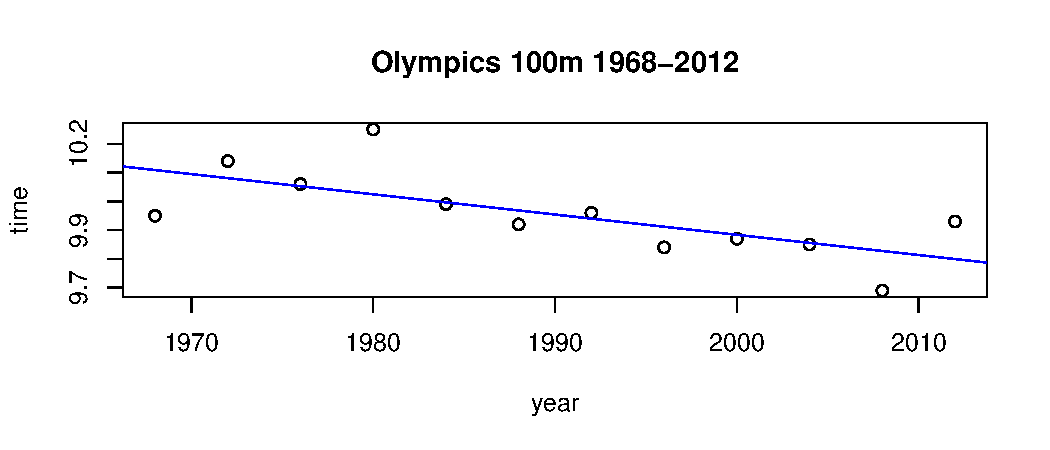
\includegraphics[width=\maxwidth]{figure/unnamed-chunk-6-1} 

\end{knitrout}
\end{frame}


\subsection[]{Step3: Construct a residual plot}
\begin{frame}[fragile]{Step3: Construct a residual plot}
A residual plot is a scatter plot of the residuals $res = e = y-(a+bx)$ vs $x$.

\vspace{.5cm}
It is a 2nd diagnostic: "Does the plot look random, or is there any pattern?"
\begin{itemize}
\item
  If the plot is random: then the LSL fit is good.
\item
	If the plot shows a relationship between $e$ and $x$, then the LSL is not adequate and we need to consider a more complex function or a transformation (eg $y=x^2$ or $y=log(x)$).
\end{itemize}
\end{frame} 
  
\begin{frame}[fragile]{}  
\begin{knitrout}
\definecolor{shadecolor}{rgb}{0.969, 0.969, 0.969}\color{fgcolor}\begin{kframe}
\begin{alltt}
\hlstd{residuals}\hlkwb{=}\hlstd{model}\hlopt{$}\hlstd{res}
\hlkwd{plot}\hlstd{(year,residuals,}\hlkwc{main}\hlstd{=}\hlstr{"Residual Plot"}\hlstd{)}
\hlkwd{abline}\hlstd{(}\hlkwc{h}\hlstd{=}\hlnum{0}\hlstd{,}\hlkwc{col}\hlstd{=}\hlstr{"red"}\hlstd{)}
\end{alltt}
\end{kframe}
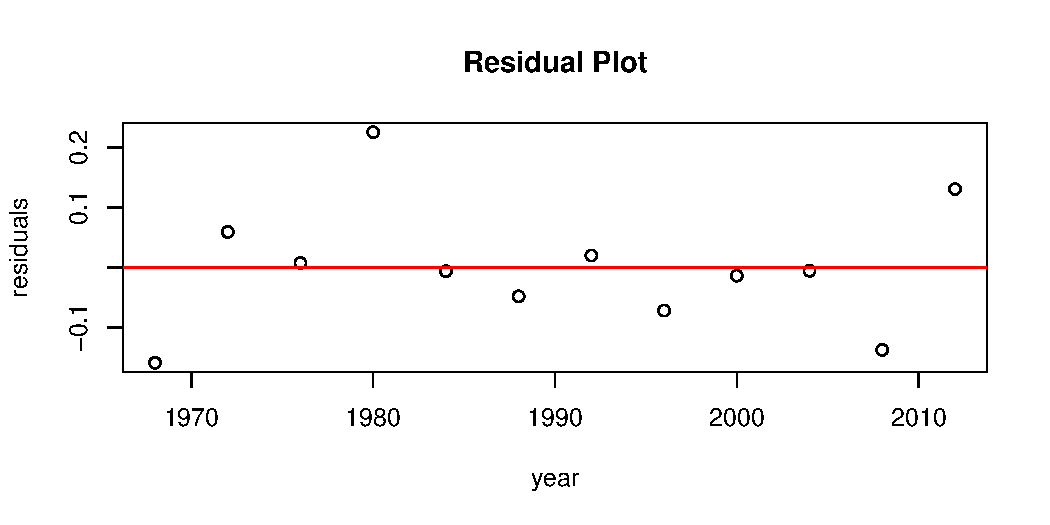
\includegraphics[width=\maxwidth]{figure/unnamed-chunk-7-1} 

\end{knitrout}
\end{frame}


\subsection[]{Step4: Calculate the correlation coefficient and the coefficient of determination}
\begin{frame}[fragile]{Step4: Calculate the correlation coefficient and the coefficient of determination}

We have calculated the ‘best’ line, but is it a good line? How strong is the linear relationship between $Y$ and $X$?

\vspace{.5cm}
A fit is considered good when the set of data points is close to the LSL, so that the residuals are small. So we consider the relationship between $s_{res}^2$ (the variance of the residuals) and $s_{y}^2$   (the variance of $y$).
\end{frame} 

\begin{frame}[fragile]{Pearson's correlation coefficient}
The correlation coefficient is
\[ \boxed{ r =  \frac{ S_{xy} }{\sqrt{ S_{xx} S_{yy}} } } \]

Properties:
\begin{itemize}
\item
$r$ is symmetric in $x$ and $y$.

\item $-1 \leq r \leq 1$ \\
$r$ is a numerical summary which indicates the strength of the linear assocation between $y$ and $x$.
\end{itemize}
\end{frame} 

\begin{frame}[fragile]{}
\begin{itemize}
\item  $r=\pm 1$ \\
This corresponds to a perfect linear correlation, with all the data points lying on the LSL.

\begin{knitrout}
\definecolor{shadecolor}{rgb}{0.969, 0.969, 0.969}\color{fgcolor}
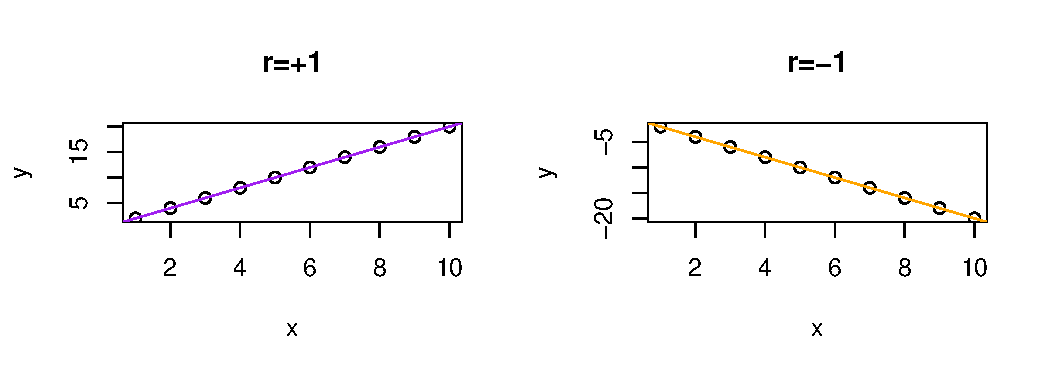
\includegraphics[width=\maxwidth]{figure/unnamed-chunk-8-1} 

\end{knitrout}
\end{itemize}
\end{frame} 

\begin{frame}[fragile]{}
\begin{itemize}
\item $r=0 $ \\
This indicates no linear correlation, for example a line with zero slope, or a random scatter, or a non linear relationship.
\end{itemize}
\begin{knitrout}
\definecolor{shadecolor}{rgb}{0.969, 0.969, 0.969}\color{fgcolor}
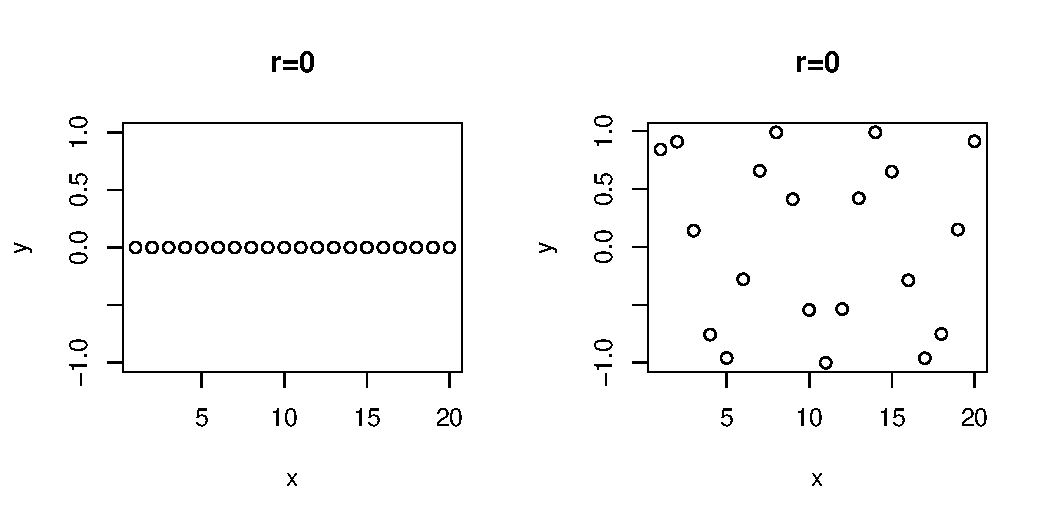
\includegraphics[width=\maxwidth]{figure/unnamed-chunk-9-1} 

\end{knitrout}
\end{frame} 

\begin{frame}[fragile]{Examples of Correlation Coefficients}
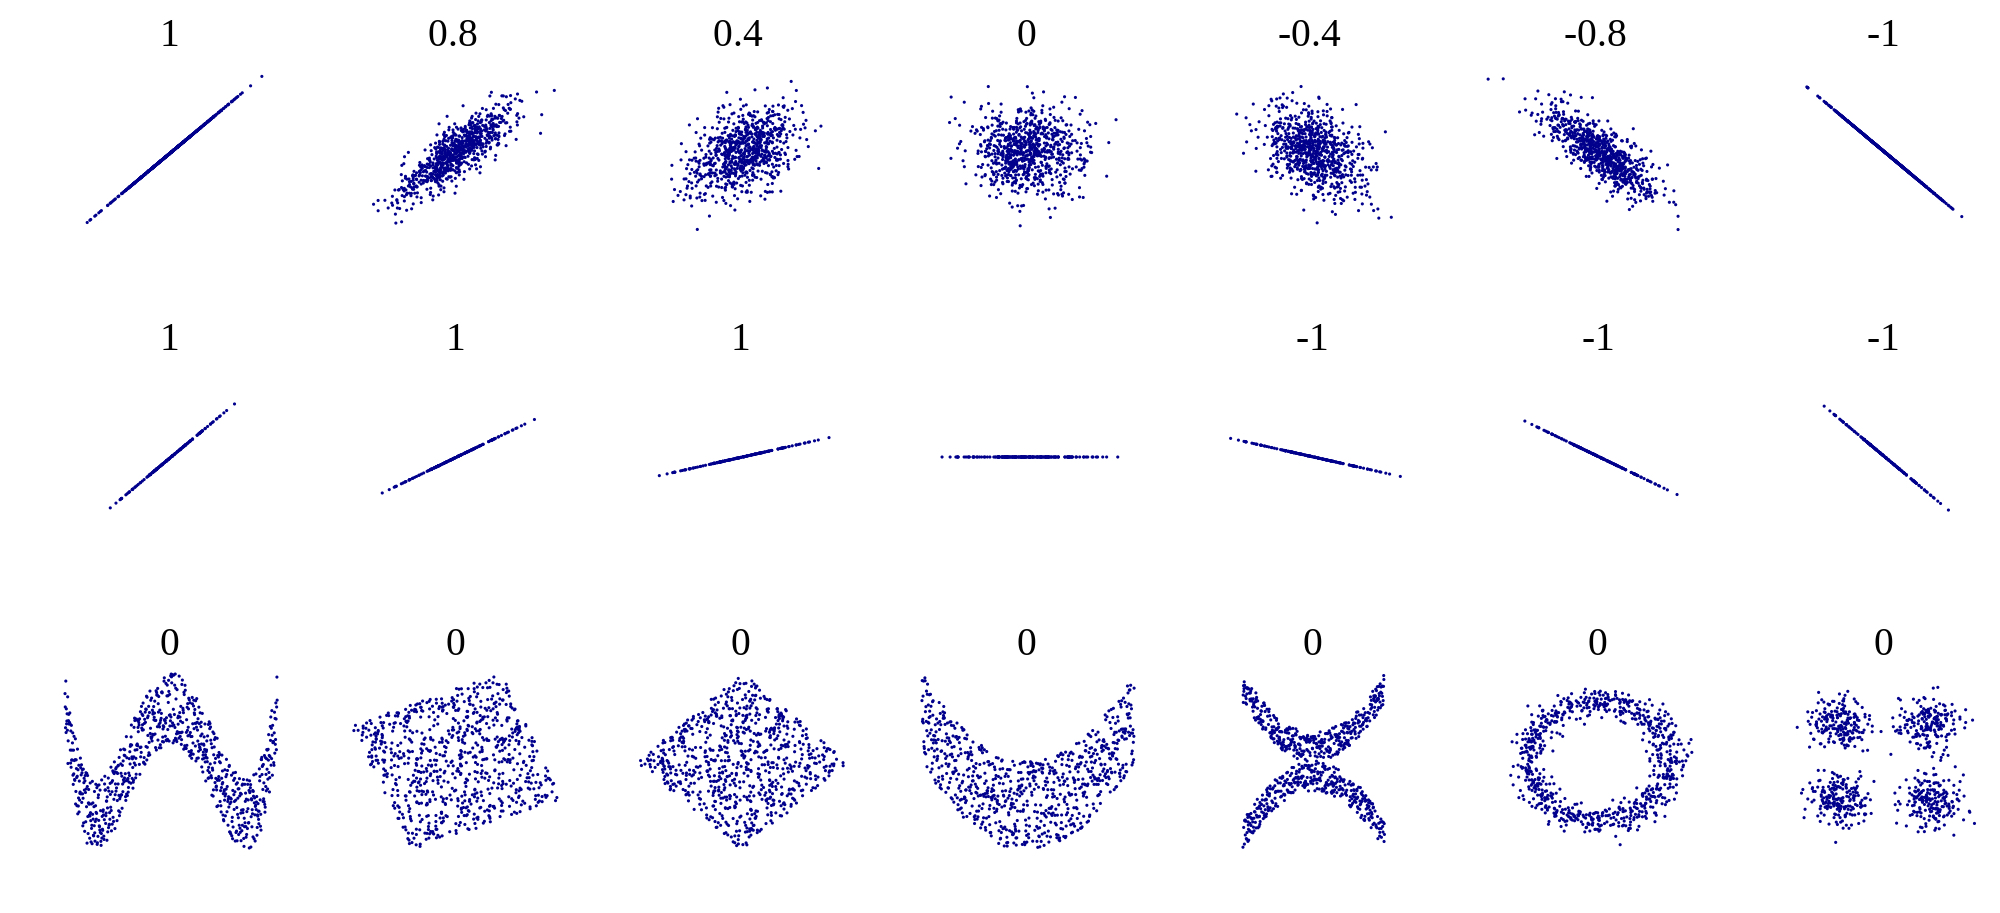
\includegraphics[height=5cm]{../images/CorrelationChart.jpg}

\href{https://en.wikipedia.org/wiki/Pearson_product-moment_correlation_coefficient}{\beamergotobutton{Link}}
\end{frame} 

\begin{frame}[fragile]{Relationship between Correlation Coefficient and Slope}
There is an interesting relationship between $r$ and $b$
\[ b =  \frac{ S_{xy} }{ S_{xx}  }
= \frac{ S_{xy} }{\sqrt{ S_{xx} S_{yy}} }   \frac{ \sqrt{ S_{yy} } }{ \sqrt{ S_{xx} } }
= r \frac{ \sqrt{ S_{yy}/(n-1)} }{ \sqrt{ S_{xx}/(n-1) }  }
= r \frac{ s_{y}}{s_{x}} \]

Hence:
\begin{itemize}
\item 
The sign of $r$ reflects the trend (slope) of the data.
\item
$r$ is unaffected by a change of scale or origin.
\end{itemize}
\end{frame} 

\begin{frame}[fragile]{The coefficient of determination}
The coefficient of determination is the proportion of variability of $y$ explained by $x$ for a model, or in our context, the proportion of variability explained by the linear regression. 

\[ \boxed{  r^2 = \frac{s_{y}^2 - s_{res}^2}{s_{y}^2} = \frac{S_{xy}^2}{S_{xx} S_{yy}}  }\]

Properties:
\begin{itemize}
\item $0 \leq r^2 \leq 1$ \\
%$r^2$ is a numerical summary: we say that $(1-r^2)100 \%$ of the variability of $y$ is explained by $x$.

\item  $r^2=1$ \\
This arises when $res_i=0 \;\; \forall i$ and $s_{res}^2=0$, ie all of the variability of the model is associated with the linear regression.
All points lie on the LSL.
\end{itemize}
\end{frame} 



\begin{frame}[fragile]{}

\begin{itemize}
\item  $r^2 \approx 1$ \\
This arises when $res_i=0$ is small compared to $s_{y}^2$, ie most of the variability of the model is associated with the linear regression.

\item $r^2=0$ \\
This arises when $s_{res}^2=s_{y}^2$, ie none the variability of the model is associated with the linear regression. 

\item $r^2 \approx 0$ \\
This arises when $s_{res}^2 \approx s_{y}^2$, ie almost none the variability of the model is associated with the linear regression. 

\item Note that $r^2$ can be small and still indicate that the model is correct (ie a model where there is naturally low association between $X$ and $Y$).

\end{itemize}
\end{frame} 

\begin{frame}[fragile]{}  
\begin{knitrout}
\definecolor{shadecolor}{rgb}{0.969, 0.969, 0.969}\color{fgcolor}\begin{kframe}
\begin{alltt}
\hlkwd{cor}\hlstd{(year,time)}
\end{alltt}
\begin{verbatim}
## [1] -0.6912573
\end{verbatim}
\begin{alltt}
\hlkwd{cor}\hlstd{(year,time)}\hlopt{^}\hlnum{2}
\end{alltt}
\begin{verbatim}
## [1] 0.4778366
\end{verbatim}
\end{kframe}
\end{knitrout}

Hence, the linear associotion between year and time for the Olympics 100m sprint is  -0.7 (fairly high). 48\% of the variation in times is explained by the variation in years.



\end{frame}



\subsection{Avoiding mistakes in Regression}
\begin{frame}[fragile]{Avoiding mistakes in Regression}

\begin{itemize}
\item Correlation does not imply causation \\
A high value of $r$ does not necessarily imply a causal relationship between $X$ and $Y$.  For example, December temperature and consumer spending).

\vspace{.5cm}
\item Causation does not imply (linear) correlation \\

\begin{knitrout}
\definecolor{shadecolor}{rgb}{0.969, 0.969, 0.969}\color{fgcolor}
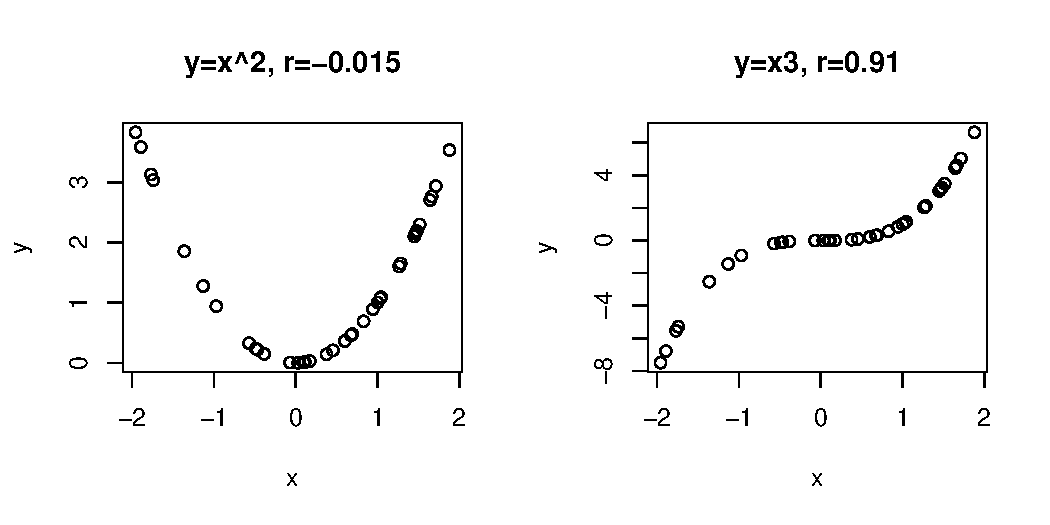
\includegraphics[width=\maxwidth]{figure/unnamed-chunk-11-1} 

\end{knitrout}
\end{itemize}
\end{frame} 


\begin{frame}[fragile]{Avoiding mistakes in Regression}
\begin{itemize}
\item The same value of $r$ can correspond to very different models.  \\

\vspace{.5cm}
The following data sets, called `Ansombe's Quartet' were constructed by Francis Anscombe in 1973. They all have $\bar{x}= 9$, $s_{x}^2=11$, $\bar{y} = 7.5$, $s_{y}^2 = 4.127$, $r=0.816$ and linear regression line $y=3+0.5x$. But look how different they look!
\end{itemize}

\href{https://en.wikipedia.org/wiki/Anscombes_quartet}{\beamergotobutton{Anscombes Quartet}}

\href{http://data.heapanalytics.com/anscombes-quartet-and-why-summary-statistics-dont-tell-the-whole-story}{\beamergotobutton{Law Grad salaries}}  %Why not work?
\end{frame} 


\begin{frame}[fragile]{}

\begin{knitrout}
\definecolor{shadecolor}{rgb}{0.969, 0.969, 0.969}\color{fgcolor}
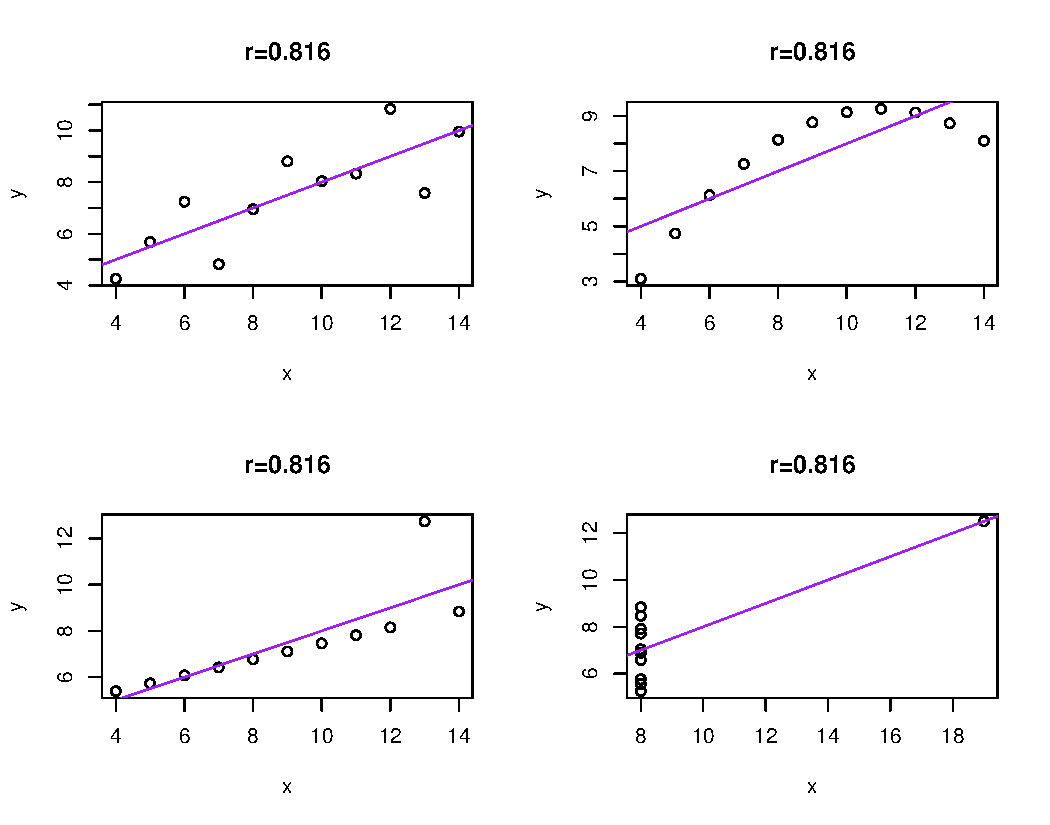
\includegraphics[width=\maxwidth]{figure/unnamed-chunk-12-1} 

\end{knitrout}
\end{frame} 


\begin{frame}[fragile]{}

\begin{itemize}
\item Even one outlier can distort the model.  \\

It's vital to draw a scatter plot before considering $r$, because of the high influence of outliers.

\begin{knitrout}
\definecolor{shadecolor}{rgb}{0.969, 0.969, 0.969}\color{fgcolor}
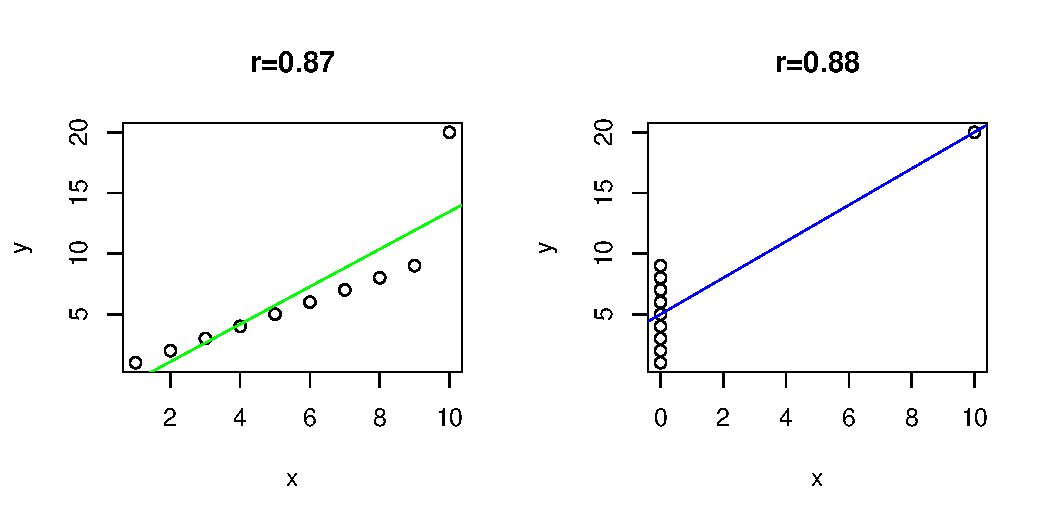
\includegraphics[width=\maxwidth]{figure/unnamed-chunk-13-1} 

\end{knitrout}
\end{itemize}
\end{frame}

\subsection{Linear regression with outliers}
\begin{frame}[fragile]{Example: Animals dataset: body vs brain weight}

Body weight in kg and brain weight in g

\begin{knitrout}
\definecolor{shadecolor}{rgb}{0.969, 0.969, 0.969}\color{fgcolor}\begin{kframe}
\begin{alltt}
\hlkwd{library}\hlstd{(MASS)} \hlcom{## The location of the package}
\hlkwd{head}\hlstd{(Animals)}
\end{alltt}
\begin{verbatim}
##                     body brain
## Mountain beaver     1.35   8.1
## Cow               465.00 423.0
## Grey wolf          36.33 119.5
## Goat               27.66 115.0
## Guinea pig          1.04   5.5
## Dipliodocus     11700.00  50.0
\end{verbatim}
\begin{alltt}
\hlkwd{names}\hlstd{(Animals)}
\end{alltt}
\begin{verbatim}
## [1] "body"  "brain"
\end{verbatim}
\end{kframe}
\end{knitrout}


\end{frame}

\begin{frame}[fragile]{Outliers galore!}
\begin{knitrout}
\definecolor{shadecolor}{rgb}{0.969, 0.969, 0.969}\color{fgcolor}
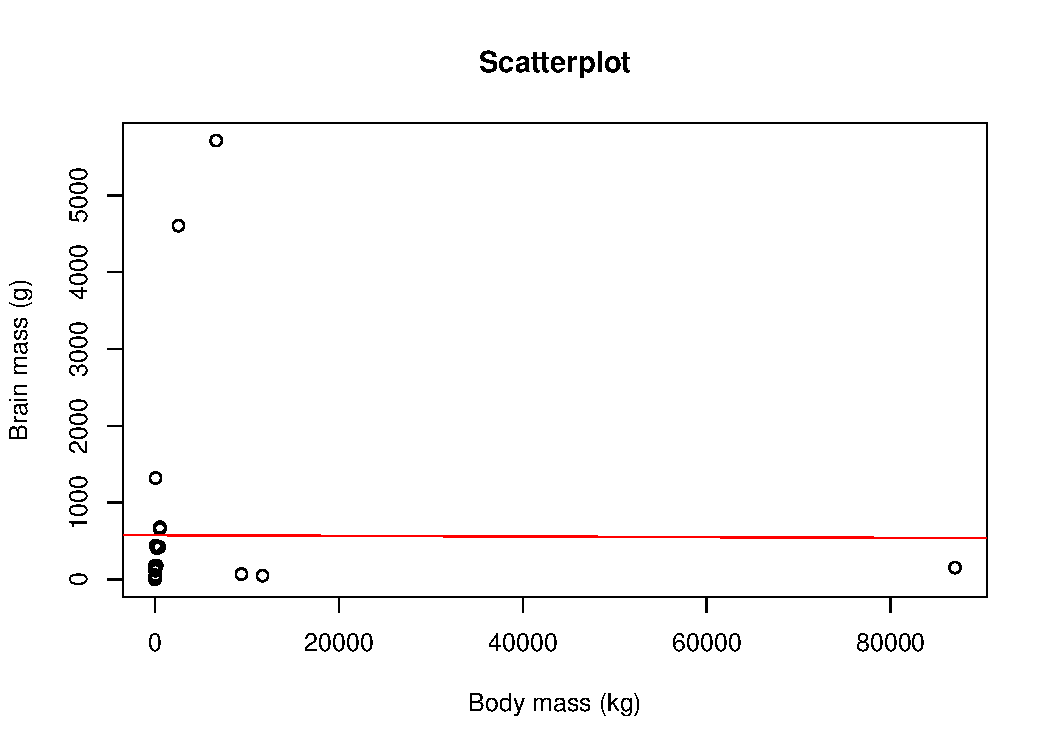
\includegraphics[width=\maxwidth]{figure/unnamed-chunk-15-1} 

\end{knitrout}
\end{frame}

\begin{frame}[fragile]{Log transformation}
\begin{knitrout}
\definecolor{shadecolor}{rgb}{0.969, 0.969, 0.969}\color{fgcolor}
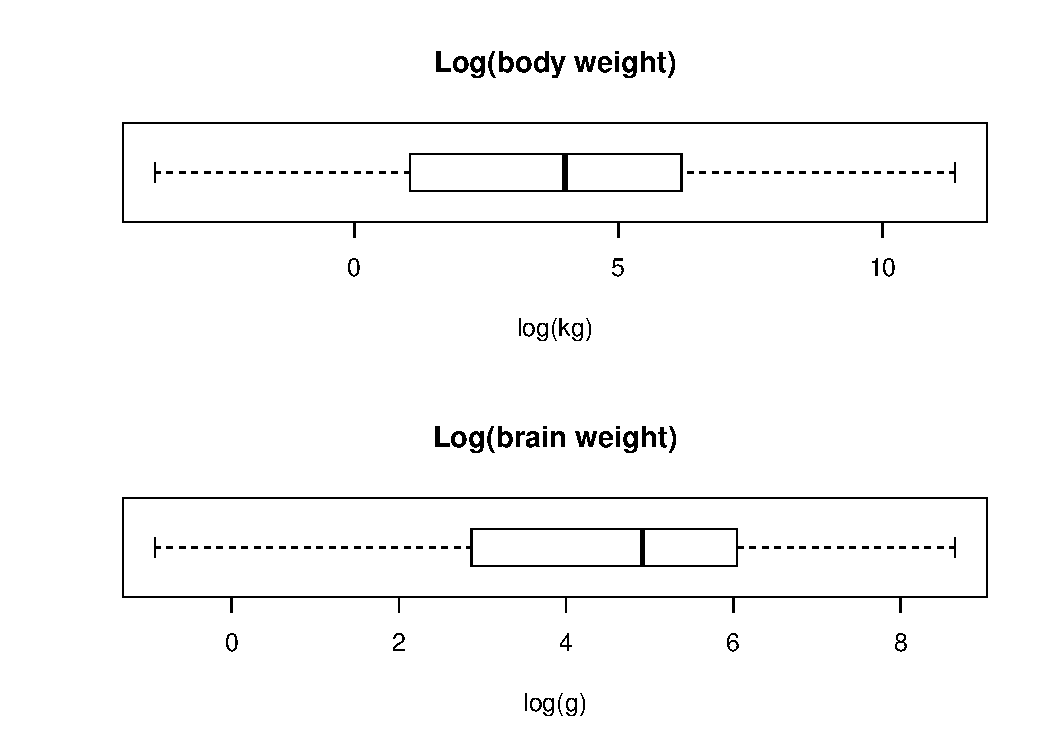
\includegraphics[width=\maxwidth]{figure/unnamed-chunk-16-1} 

\end{knitrout}
\end{frame}

\begin{frame}[fragile]{Log transformation linear regression}
\begin{knitrout}
\definecolor{shadecolor}{rgb}{0.969, 0.969, 0.969}\color{fgcolor}
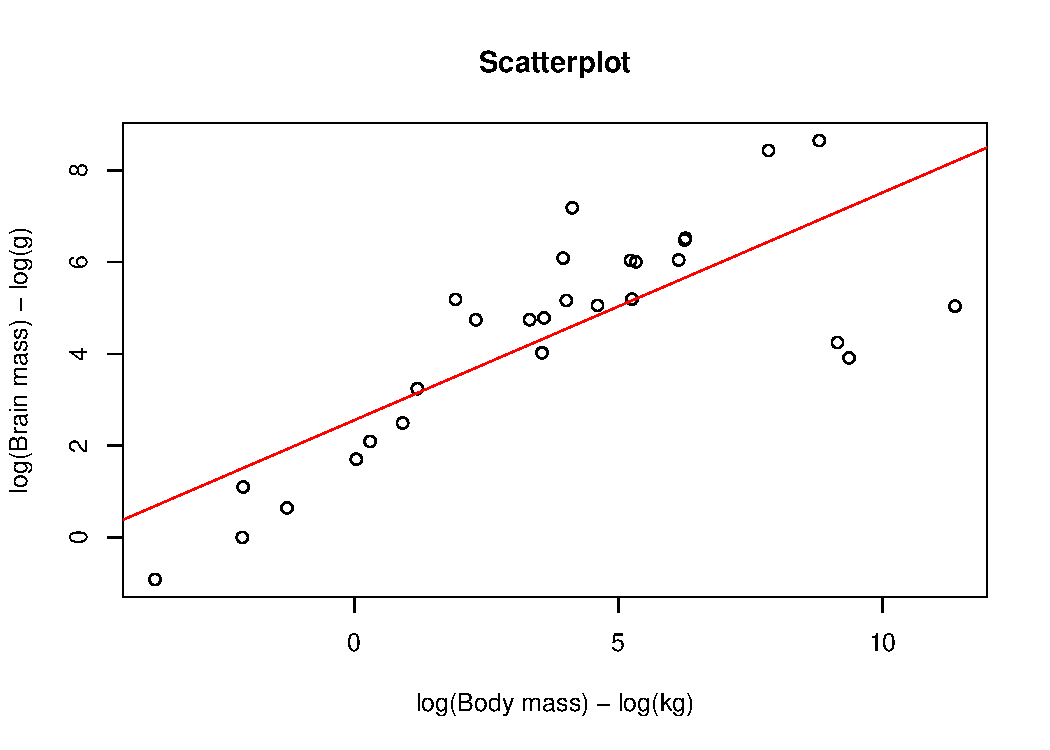
\includegraphics[width=\maxwidth]{figure/unnamed-chunk-17-1} 

\end{knitrout}
\end{frame}

\begin{frame}[fragile]{Robust regression}
\begin{knitrout}
\definecolor{shadecolor}{rgb}{0.969, 0.969, 0.969}\color{fgcolor}
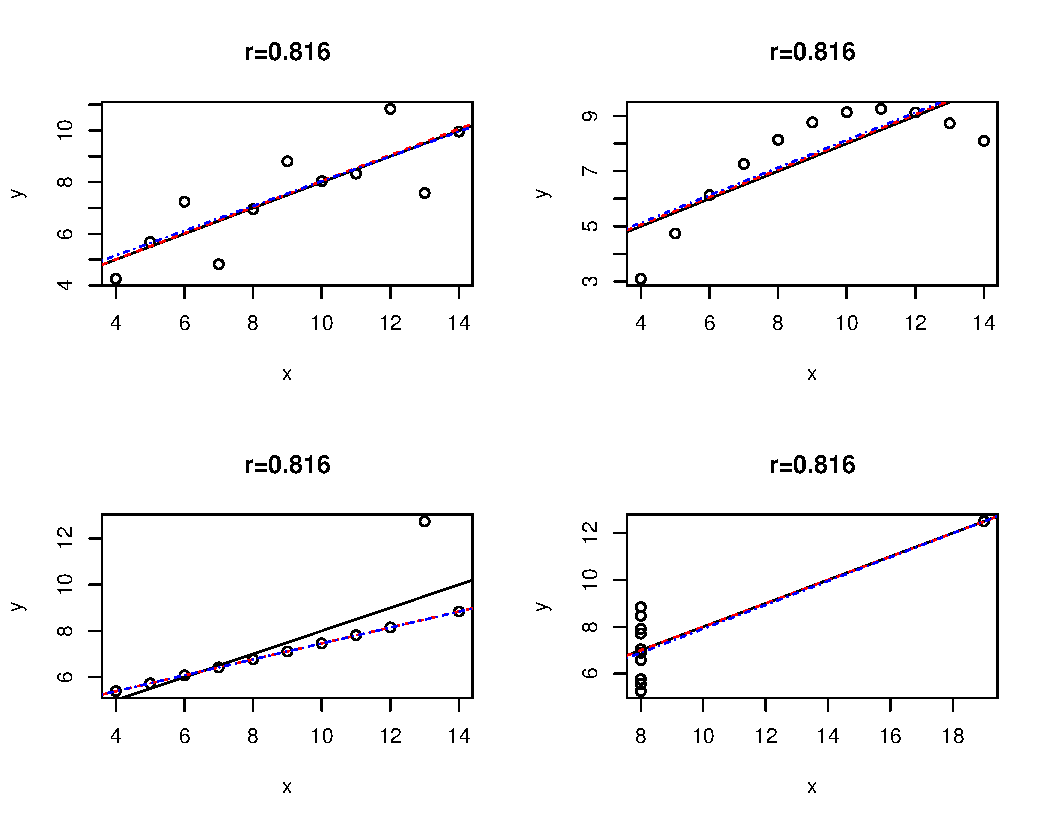
\includegraphics[width=\maxwidth]{figure/unnamed-chunk-18-1} 

\end{knitrout}
\end{frame}

\begin{frame}[fragile]{Robust regression}
\begin{knitrout}
\definecolor{shadecolor}{rgb}{0.969, 0.969, 0.969}\color{fgcolor}
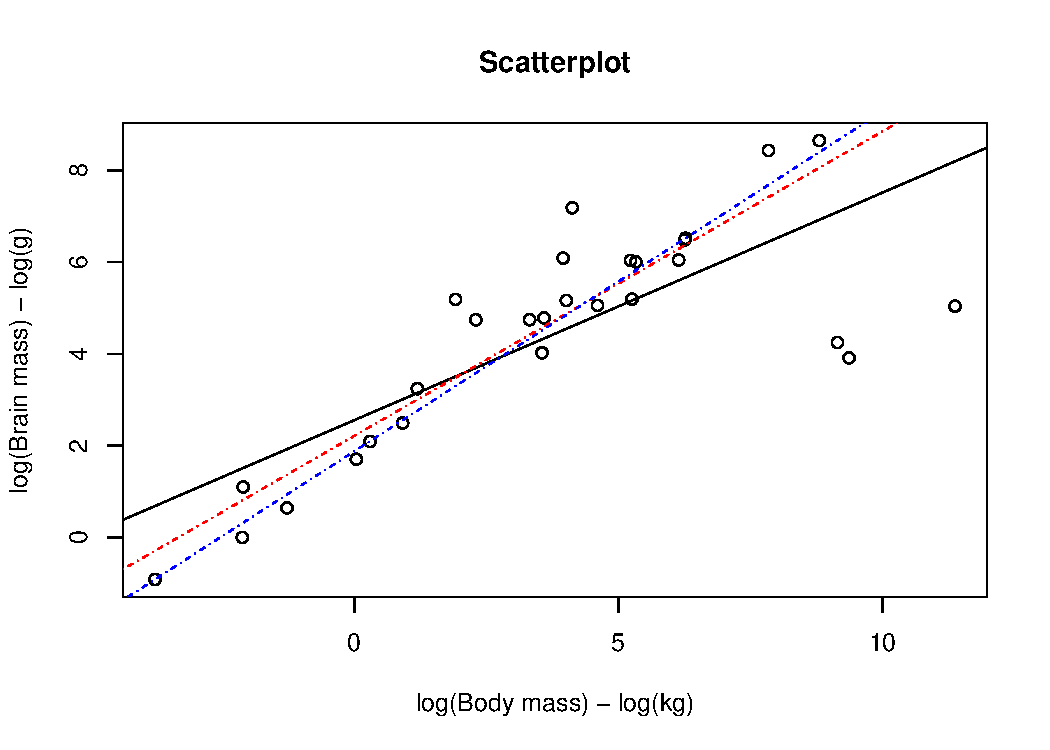
\includegraphics[width=\maxwidth]{figure/unnamed-chunk-19-1} 

\end{knitrout}
\end{frame}

\begin{frame}[fragile]{In R}
The red line is MM regression
\begin{knitrout}
\definecolor{shadecolor}{rgb}{0.969, 0.969, 0.969}\color{fgcolor}\begin{kframe}
\begin{alltt}
\hlkwd{library}\hlstd{(MASS)}   \hlcom{# library}
\hlkwd{plot}\hlstd{(x, y)}
\hlstd{red_line} \hlkwb{=} \hlkwd{rlm}\hlstd{(y}\hlopt{~}\hlstd{x)}  \hlcom{# r[obust]lm()}
\hlkwd{abline}\hlstd{(red_line,} \hlkwc{col}\hlstd{=}\hlstr{"red"}\hlstd{)}
\end{alltt}
\end{kframe}
\end{knitrout}
The blue line is quantile regression
\begin{knitrout}
\definecolor{shadecolor}{rgb}{0.969, 0.969, 0.969}\color{fgcolor}\begin{kframe}
\begin{alltt}
\hlkwd{library}\hlstd{(quantreg)}   \hlcom{# library}
\hlkwd{plot}\hlstd{(x, y)}
\hlstd{blue_line} \hlkwb{=} \hlkwd{rq}\hlstd{(y}\hlopt{~}\hlstd{x)}  \hlcom{# r[egression]q[uantile]()}
\hlkwd{abline}\hlstd{(blue_line,} \hlkwc{col}\hlstd{=}\hlstr{"blue"}\hlstd{)}
\end{alltt}
\end{kframe}
\end{knitrout}
\end{frame}

\end{document}
